\documentclass[
	% -- opções da classe memoir --
	12pt,				% tamanho da fonte
	%openright,			% capítulos começam em pág ímpar (insere página vazia caso preciso)
	oneside,			% para impressão no anverso. Oposto a twoside
	a4paper,			% tamanho do papel. 
	% -- opções da classe abntex2 --
	chapter=TITLE,		% títulos de capítulos convertidos em letras maiúsculas
	section=TITLE,		% títulos de seções convertidos em letras maiúsculas
	%subsection=TITLE,	% títulos de subseções convertidos em letras maiúsculas
	%subsubsection=TITLE,% títulos de subsubseções convertidos em letras maiúsculas
	% -- opções do pacote babel --
	english,			% idioma adicional para hifenização
	%french,				% idioma adicional para hifenização
	%spanish,			% idioma adicional para hifenização
	brazil				% o último idioma é o principal do documento
	]{abntex2}

\usepackage{setup/ufscthesisA4-alf}

% ---
% Filtering and Mapping Bibliographies
% ---
% Pacotes de citações
% ---
\usepackage{csquotes}
\usepackage[backend = biber, style = abnt]{biblatex}
% FIXME Se desejar estilo numérico de citações,  comente a linha acima e descomente a linha a seguir.
% \usepackage[backend = biber, style = numeric-comp]{biblatex}

\setlength\bibitemsep{\baselineskip}
\DeclareFieldFormat{url}{Disponível~em:\addspace\url{#1}}
\NewBibliographyString{sineloco}
\NewBibliographyString{sinenomine}
\DefineBibliographyStrings{brazil}{%
	sineloco     = {\mkbibemph{S\adddot l\adddot}},
	sinenomine   = {\mkbibemph{s\adddot n\adddot}},
	andothers    = {\mkbibemph{et\addabbrvspace al\adddot}},
	in			 = {\mkbibemph{In:}}
}

\addbibresource{aftertext/references.bib} % Seus arquivos de referências

% ---
\DeclareSourcemap{
	\maps[datatype=bibtex]{
		% remove fields that are always useless
		\map{
			\step[fieldset=abstract, null]
			\step[fieldset=pagetotal, null]
		}
		% remove URLs for types that are primarily printed
%		\map{
%			\pernottype{software}
%			\pernottype{online}
%			\pernottype{report}
%			\pernottype{techreport}
%			\pernottype{standard}
%			\pernottype{manual}
%			\pernottype{misc}
%			\step[fieldset=url, null]
%			\step[fieldset=urldate, null]
%		}
		\map{
			\pertype{inproceedings}
			% remove mostly redundant conference information
			\step[fieldset=venue, null]
			\step[fieldset=eventdate, null]
			\step[fieldset=eventtitle, null]
			% do not show ISBN for proceedings
			\step[fieldset=isbn, null]
			% Citavi bug
			\step[fieldset=volume, null]
		}
	}
}
% ---

% ---
% Informações de dados para CAPA e FOLHA DE ROSTO
% ---
\autor{Felipe Eduardo Piccini Dal Magro \\
        Gabriela Beatriz Rigo Wietzkoski\\
        Rafael Haas Ferracini 
        }
\titulo{Experimento 4: Movimento retilíneo uniforme}
%\subtitulo{Subtítulo (se houver}
\orientador{Prof. Celso Yuji Matuo e Gerson Renzetti Ouriques}
% \orientador[Orientadora]{Nome da orientadora, Dra.}
% \coorientador{Prof. XXXXXX, Dr.}
% \coorientador[Coorientadora]{XXXXXX, Dra.}
% \coordenador{Prof. XXXXXX, Dr.}
% \coordenador[Coordenadora]{Nome da Coordenadora, Dra.}
\ano{2023}
\data{23 de Outubro de 2023}
\local{Florianópolis}
\instituicaosigla{UFSC}
\instituicao{Universidade Federal de Santa Catarina}
\tipotrabalho{Relatório}
%\formacao{[licenciado/bacharel] em [nome do título obtido]}
%\nivel{[licenciado/bacharel]}
\programa{Curso de Graduação em Física}
\centro{Centro de Ciências Físicas e Matemáticas}
\preambulo
{% Modifiquei muito essa parte, revisar código original para mudanças
Relatório de Experimento 5 da disciplina de Laboratório de Física I
}
% ---

% ---
% Configurações de aparência do PDF final
% ---
% alterando o aspecto da cor azul
\definecolor{blue}{RGB}{41,5,195}
% informações do PDF
\makeatletter
\hypersetup{
     	%pagebackref=true,
		pdftitle={\@title}, 
		pdfauthor={\@author},
    	pdfsubject={\imprimirpreambulo},
	    pdfcreator={LaTeX with abnTeX2},
		pdfkeywords={ufsc, latex, abntex2}, 
		colorlinks=true,       		% false: boxed links; true: colored links
    	linkcolor=black,%blue,          	% color of internal links
    	citecolor=black,%blue,        		% color of links to bibliography
    	filecolor=black,%magenta,      		% color of file links
		urlcolor=black,%blue,
		bookmarksdepth=4
}
\makeatother
% ---

% ---
% compila a lista de abreviaturas e siglas e a lista de símbolos
% ---

% Declaração das siglas
\siglalista{ABNT}{Associação Brasileira de Normas Técnicas}

% Declaração dos simbolos
\simbololista{C}{\ensuremath{C}}{Circunferência de um círculo}
\simbololista{pi}{\ensuremath{\pi}}{Número pi} 
\simbololista{r}{\ensuremath{r}}{Raio de um círculo}
\simbololista{A}{\ensuremath{A}}{Área de um círculo}

% compila a lista de abreviaturas e siglas e a lista de símbolos
\makenoidxglossaries 

% ---

% ---
% compila o indice
% ---
\makeindex
% ---

% ----
% Início do documento
% ----
\begin{document}

% Seleciona o idioma do documento (conforme pacotes do babel)
%\selectlanguage{english}
\selectlanguage{brazil}

% Retira espaço extra obsoleto entre as frases.
\frenchspacing 

% Espaçamento 1.5 entre linhas
\OnehalfSpacing

% Corrige justificação
%\sloppy

% ----------------------------------------------------------
% ELEMENTOS PRÉ-TEXTUAIS
% ----------------------------------------------------------
% \pretextual %a macro \pretextual é acionado automaticamente no início de \begin{document}
% ---
% Capa, folha de rosto, ficha bibliografica, errata, folha de apróvação
% Dedicatória, agradecimentos, epígrafe, resumos, listas
% ---
\imprimircapa
%% ---
% Capa
% ---
\imprimircapa
% ---

% ---
% Folha de rosto
% (o * indica que haverá a ficha bibliográfica)
% ---
%\imprimirfolhaderosto*
% ---

% ---
% Inserir a ficha bibliografica
% ---
% http://ficha.bu.ufsc.br/
%\begin{fichacatalografica}
%	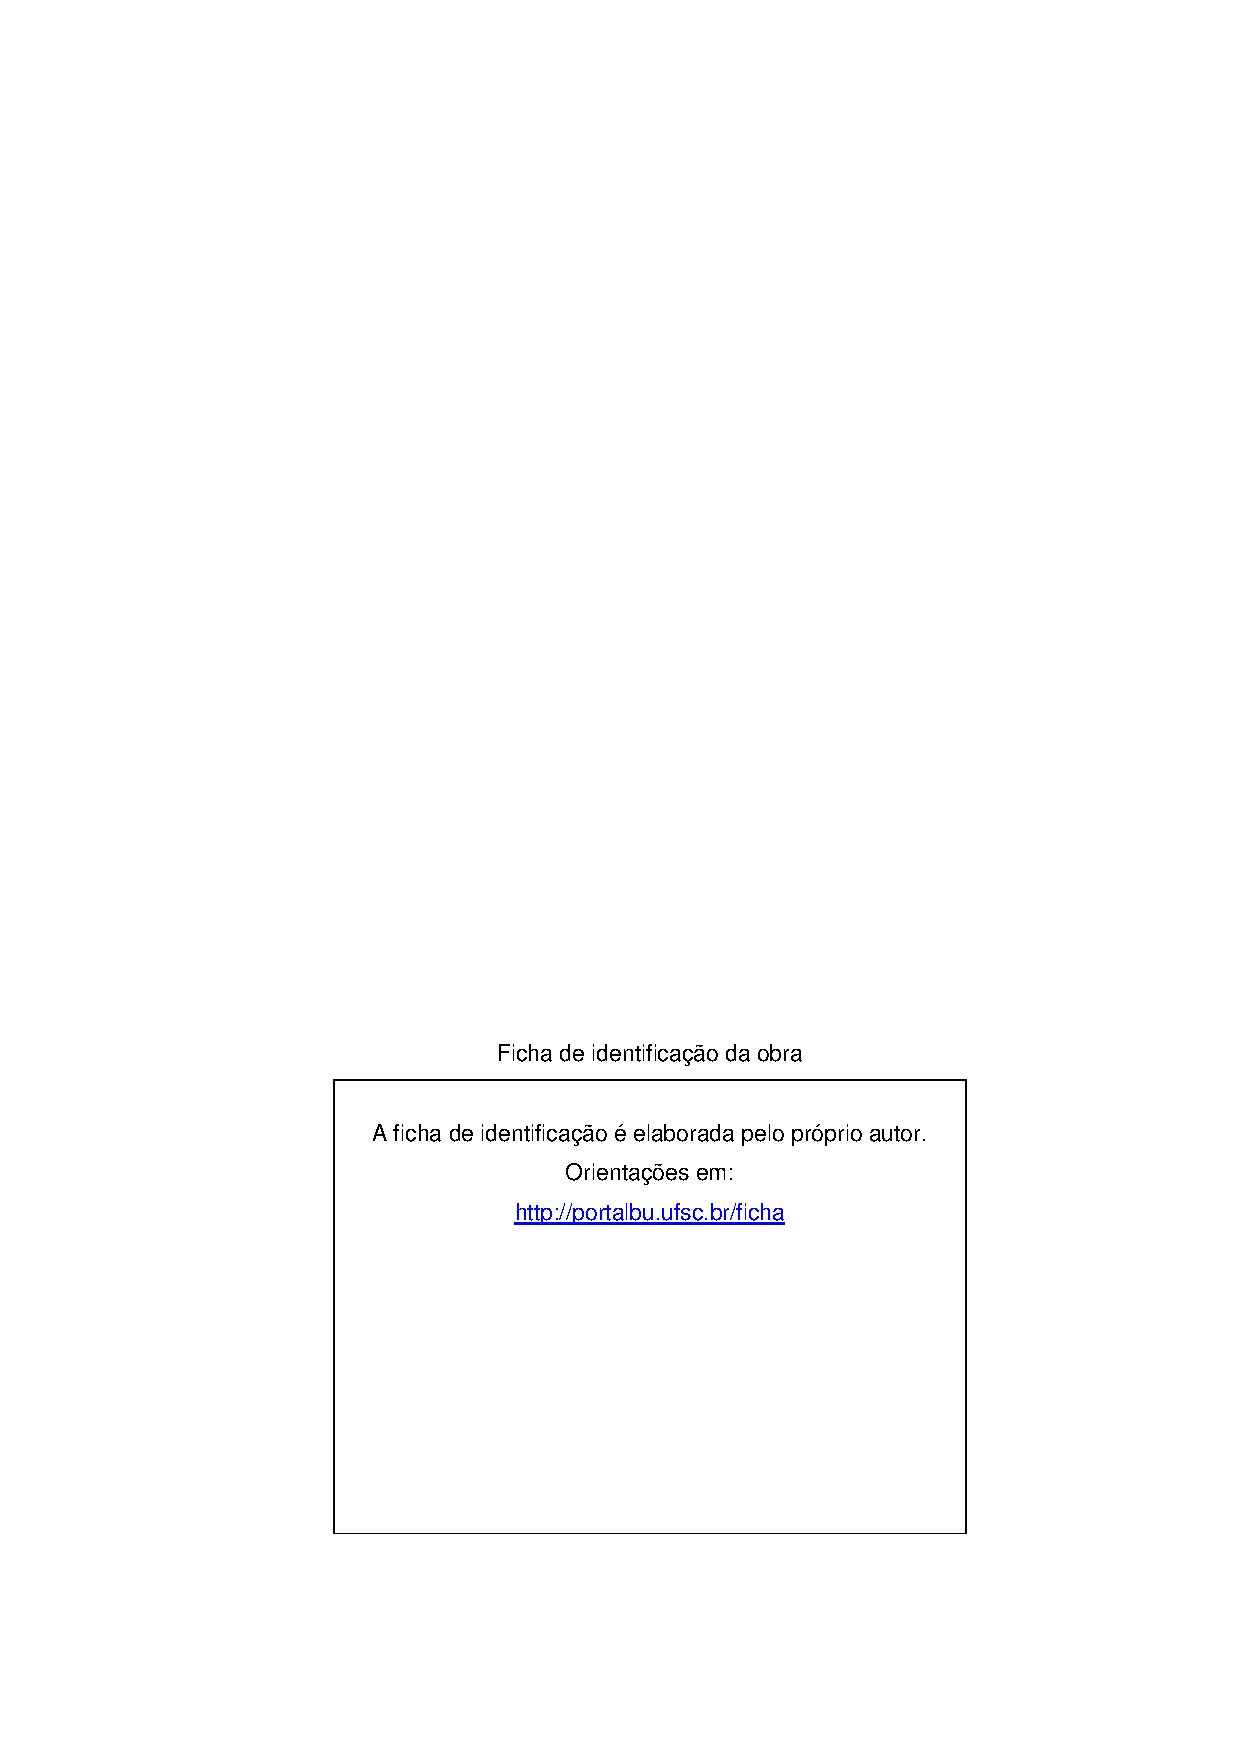
\includepdf{beforetext/Ficha_Catalografica.pdf}
%\end{fichacatalografica}
% ---

% ---
% Inserir folha de aprovação
% ---
%\begin{folhadeaprovacao}
%	\OnehalfSpacing
%	\centering
%	\imprimirautor\\%
%	\vspace*{10pt}		
%	\textbf{\imprimirtitulo}%
%	\ifnotempty{\imprimirsubtitulo}{:~\imprimirsubtitulo}\\%
%	%		\vspace*{31.5pt}%3\baselineskip
%	\vspace*{\baselineskip}
%	%\begin{minipage}{\textwidth}
%	% ~do~\imprimirprograma~do~\imprimircentro~da~\imprimirinstituicao~para~a~obtenção~do~título~de~\imprimirformacao.
%	Este~\imprimirtipotrabalho~foi julgado adequado para obtenção do Título de “\imprimirformacao” e aprovado em sua forma final pelo~\imprimirprograma. \\
%		\vspace*{\baselineskip}
%	\imprimirlocal, \imprimirdata. \\
%	\vspace*{2\baselineskip}
%	\assinatura{\OnehalfSpacing\imprimircoordenador \\ \imprimircoordenadorRotulo~do Curso}
%	\vspace*{2\baselineskip}
%	\textbf{Banca Examinadora:} \\
%	\vspace*{\baselineskip}
%	\assinatura{\OnehalfSpacing\imprimirorientador \\ \imprimirorientadorRotulo}
	%\end{minipage}%
%	\vspace*{\baselineskip}
%	\assinatura{Prof.(a) xxxx, Dr(a).\\
%	Avaliador(a) \\
%	Instituição xxxx}

%	\vspace*{\baselineskip}
%	\assinatura{Prof.(a) xxxx, Dr(a).\\
%	Avaliador(a) \\
%	Instituição xxxx}
%\end{folhadeaprovacao}
% ---

% ---
% Dedicatória
% ---
%\begin{dedicatoria}
%	\vspace*{\fill}
%	\noindent
%	\begin{adjustwidth*}{}{5.5cm}     
%		Este trabalho é dedicado aos meus colegas de classe e aos meus queridos pais.
%	\end{adjustwidth*}
%\end{dedicatoria}
% ---

% ---
% Agradecimentos
% ---
%\begin{agradecimentos}
%	Inserir os agradecimentos aos colaboradores à execução do trabalho. 
%	
%	Xxxxxxxxxxxxxxxxxxxxxxxxxxxxxxxxxxxxxxxxxxxxxxxxxxxxxxxxxxxxxxxxxxxxxx. 
%\end{agradecimentos}
% ---

% ---
% Epígrafe
% ---
%\begin{epigrafe}
%	\vspace*{\fill}
%	\begin{flushright}
%		\textit{``Texto da Epígrafe.\\
%			Citação relativa ao tema do trabalho.\\
%			É opcional. A epígrafe pode também aparecer\\
%			na abertura de cada seção ou capítulo.\\
%			Deve ser elaborada de acordo com a NBR 10520.''\\
%			(Autor da epígrafe, ano)}
%	\end{flushright}
%\end{epigrafe}
% ---

% ---
% RESUMOS
% ---

% resumo em português
%\setlength{\absparsep}{18pt} % ajusta o espaçamento dos parágrafos do resumo
%\begin{resumo}
%	\SingleSpacing
%	Resumo
%	
%	\textbf{Palavras-chave}: Palavra-chave 1. Palavra-chave 2. Palavra-chave 3.
%\end{resumo}

% resumo em inglês
%\begin{resumo}[Abstract]
%	\SingleSpacing
%	\begin{otherlanguage*}{english}
%		Translate 
%		
%		\textbf{Keywords}: Keyword 1. Keyword 2. Keyword 3.
%	\end{otherlanguage*}
%\end{resumo}

%% resumo em francês 
%\begin{resumo}[Résumé]
% \begin{otherlanguage*}{french}
%    Il s'agit d'un résumé en français.
% 
%   \textbf{Mots-clés}: latex. abntex. publication de textes.
% \end{otherlanguage*}
%\end{resumo}
%
%% resumo em espanhol
%\begin{resumo}[Resumen]
% \begin{otherlanguage*}{spanish}
%   Este es el resumen en español.
%  
%   \textbf{Palabras clave}: latex. abntex. publicación de textos.
% \end{otherlanguage*}
%\end{resumo}
%% ---

{%hidelinks
	\hypersetup{hidelinks}
	% ---
	% inserir lista de ilustrações
	% ---
	\pdfbookmark[0]{\listfigurename}{lof}
	\listoffigures*
	\cleardoublepage
	% ---
	
	% ---
	% inserir lista de quadros
	% ---
	%\pdfbookmark[0]{\listofquadrosname}{loq}
	%\listofquadros*
	%\cleardoublepage
	% ---
	
	% ---
	% inserir lista de tabelas
	% ---
	\pdfbookmark[0]{\listtablename}{lot}
	\listoftables*
	\cleardoublepage
	% ---
	
	% ---
	% inserir lista de abreviaturas e siglas (devem ser declarados no preambulo)
	% ---
	%\imprimirlistadesiglas
	% ---
	
	% ---
	% inserir lista de símbolos (devem ser declarados no preambulo)
	% ---
	%\imprimirlistadesimbolos
	% ---
	
	% ---
	% inserir o sumario
	% ---
	\pdfbookmark[0]{\contentsname}{toc}
	\tableofcontents*
	\cleardoublepage
	
}%hidelinks
% ---

% ---

% ----------------------------------------------------------
% ELEMENTOS TEXTUAIS
% ----------------------------------------------------------
\textual

% ---
% 1 - Introdução
% ---
% ----------------------------------------------------------
\chapter{Dados experimentais}\label{cap:dados_experimentais}
% ----------------------------------------------------------
\section{Experimento 1}

\begin{table}[h]
\centering
\begin{tabular}{ |m{1cm}|m{3cm}|m{3cm}|  } 
\hline
\multicolumn{3}{|c|}{Dados experimentais experiência 1} \\
\hline
 & Posição x (cm) & Tempo t (s) \\
\hline
$x_0$ & $30,00 \pm 0,05$ & $0$ \\
$x_1$ & $45,00 \pm 0,05$ & $0,309 \pm 0,001$ \\
$x_2$ & $60,00 \pm 0,05$ & $0,604 \pm 0,001$ \\
$x_3$ & $75,00 \pm 0,05$ & $0,919 \pm 0,001$ \\
$x_4$ & $90,00 \pm 0,05$ & $1,259 \pm 0,001$ \\
$x_5$ & $105,00 \pm 0,05$ & $1,591 \pm 0,001$   \\
$x_6$ & $120,00 \pm 0,05$ & $1,917 \pm 0,001$ \\
$x_7$ & $135,00 \pm 0,05$ & $2,239 \pm 0,001$ \\
$x_8$ & $150,00 \pm 0,05$ & $2,391 \pm 0,001$ \\
$x_9$ & $165,00 \pm 0,05$ & $2,833 \pm 0,001$ \\
$x_{10}$ & $180,00 \pm 0,05$ & $3,141 \pm 0,001$ \\
\hline
\end{tabular}
\caption{Dados experimentais}
\label{table:experimento1}
\end{table}

\section{Experimento 2}

\begin{table}[h]
    \centering
    \begin{tabular}{|c|c|}
        \hline
        P & $\left(100,00 \pm 0,05\right)cm$ \\
        \hline 
        L & $\left(9,975 \pm 0,0005\right)cm$ \\
        \hline
    \end{tabular}
    \caption{Medida do instrumento}
    \label{tab:instrumentos}
\end{table}

\begin{table}[h]
    \centering
    \begin{tabular}{|c|}
        \hline
        $t_l (s)$ \\
        \hline
        $0,222 \pm 0,001$ \\
        \hline
        $0,210 \pm 0,001$ \\
        \hline
        $0,205 \pm 0,001$ \\
        \hline
        $0,215 \pm 0,001$ \\
        \hline
        $0,218 \pm 0,001$ \\
        \hline
    \end{tabular}
    \caption{Medida de tempo}
    \label{tab:tempos}
\end{table}


% ---

% ---
% 2 - Capítulo 2
% ---
% ----------------------------------------------------------
\chapter{Análise gráfica}\label{cap:analise_grafica}
% ----------------------------------------------------------
\section{Linearização}
Tomando a equação horária da posição do movimento retilíneo uniforme
\begin{equation}\label{eq: funcao_horaria}
    x(t) = x_0 + v_x t
\end{equation}

Estamos interessados em tomar $t$ como variável dependente e $x$ como variável independente. Isolando t na \autoref{eq: funcao_horaria} temos
\begin{equation*}
    t = \frac{1}{v_x}x - \frac{x_0}{v_x}
\end{equation*}

Conseguimos então linearizar com uma equação da forma $Y = A + BX$ tomando
\begin{equation}\label{eq: linearizacao}
    t = \frac{1}{v_x}x - \frac{x_0}{v_x} \Rightarrow \left\{ \begin{array}{ll}
        Y = t &  \\
        X = x &  \\
        A = -\frac{x_0}{v_x} & \\
        B = \frac{1}{v_x}
    \end{array}\right.
\end{equation}

\section{Gráfico}
Com o auxílio do programa SciDAVis podemos plotar os dados da \autoref{table:experimento1} e obter a regressão linear com os respectivos coeficientes linear ($A = -0,629 \pm 0,0332712893656291$) e angular ($B =  0,0208848484848485 \pm 0,000288770195295941$) e seus erros, explicitado na \autoref{fig:grafico}.
\begin{figure}[htb]
	\caption{\label{fig:grafico}Gráfico do tempo em função do deslocamento}
	\begin{center}
		\includegraphics[width=10cm]{images/experimento5_grafico.png}
	\end{center}
	\fonte{Autoral.}
\end{figure}

% ---

% ---
% 3 - Capítulo 3
% ---
% ----------------------------------------------------------
\chapter{Questionário}\label{cap:questionario}
% ----------------------------------------------------------

\begin{enumerate}
    \item 
    \begin{enumerate}
        \item \textbf{A partir dos valores obtidos para os parâmetros da melhor reta, determine os valores experimentais de $x_0$ e de $v_x$, com suas respectivas unidades de medida.} 
        
        Utilizando a linearização obtida na \autoref{eq: linearizacao}, com o coeficiente angular (B) podemos obter o valor de $v_x$.
        \begin{equation}\label{eq:vx}
            v_x = \frac{1}{B} \therefore v_x = 47,8816018572257343 \frac{cm}{s}
        \end{equation}

        O valor para $x_0$ podemos obter a partir do coeficiente linear A.
        \begin{equation}\label{eq:x0}
            x_0 = -A v_x \therefore x_0 = 30,1175275681949868 cm
        \end{equation}

        \item \textbf{ Com o auxílio do computador, determine o erro no parâmetro angular B, e através deste o erro na velocidade $v_x$}

        Para obter o valor do erro, usamos as expressões para $v_x$ e $x_0$ obtida na \autoref{eq:vx} e \autoref{eq:x0}.

        Para $dv_x$ temos:

        \begin{align}
            dv_x &= \left\| \frac{\partial v_x}{\partial B}\right\| dB = \left\|\frac{\partial}{\partial B} \left(\frac{1}{B}\right)\right\| dB = \frac{1}{B^2} dB \\
            \therefore dv_x &= 0,6620483519152457 \frac{cm}{s}
        \end{align}

        \begin{equation}
            \therefore v_x = \left(47,9 \pm 0,7 \right) \frac{cm}{s}
        \end{equation}

        \item \textbf{O valor de $x_0$ era o esperado? Justifique sua resposta.}\\
        Sim, é um valor esperado. O valor $x_0 \approx 30,12$ deu muito próximo do que no experimento foi tomado como posição inicial para o primeiro detector.
    \end{enumerate}

    \item
    \begin{enumerate}
        \item \textbf{Por que razão costumamos dizer que, na prática, é difícil obtermos um movimento retilíneo uniforme?} \\
        Um dos motivos é a dificuldade de isolar um sistema de forças externas. Forças de ação a distâncias não podem ser restringidas por nenhum tipo de barreira; forças dissipativas (resistência do ar, atrito) estão presentes em quaisquer equipamentos; condições ambiente também podem alterar os resultados.
        

        \item \textbf{Cite um exemplo da vida real em que o movimento pode ser considerado movimento retilíneo uniformes.}\\
        Um satélite orbitando em volta da Terra (como sistema de GPS, analises climáticas); uma gota de chuva ao atingir velocidade terminal
    \end{enumerate}

    \item 
    \begin{enumerate}
        \item \textbf{Com base nos dados constantes na tabela referente à Parte II de suas medidas, calcule a velocidade do carrinho com o respectivo erro propagado. Lembre-se que, no caso da medida do comprimento da bandeirola, consideramos apenas o erro de escala, mas na medida do tempo devemos considerar não apenas este último como também o erro aleatório} \\

        \begin{enumerate}
            \item Calculando primeiro a expressão para a velocidade e seu erro
            Sabemos da cinemática que
            \begin{equation} \label{eq: v_med}
                v_{carro} = \frac{x}{t}
            \end{equation}
    
            Pela teoria de propagação de erro, o erro dessa operação será dado por
            \begin{equation*}
                dv = \left\| \frac{\partial v}{\partial x}\right\| dx + \left\| \frac{\partial v}{\partial t}\right\| dt 
            \end{equation*}
            \begin{equation} \label{eq:erro_vmed}
                \therefore dv = \frac{1}{t} dx + \frac{x}{t^2} dt
            \end{equation}

            \item Calcular o tempo médio medido

            \begin{equation}
                \bar{t} = \frac{0,222 + 0,210 + 0,205 + 0,215 + 0,218}{5} \therefore \bar{t} = 0,214s
            \end{equation}

            \item Calcular o Desvio Padrão 

            \begin{equation}
                \sigma = \sqrt{\frac{\sum_{i=1}^N \left(t_i - \bar{t}\right)^2 }{N}} \therefore \sigma = 0,005967s
            \end{equation}

            \item Calcular o Erro Aleatório Provável
            \begin{equation}
                \sigma_{med} = \frac{\sigma}{\sqrt{N}} \therefore \sigma_{med} = 0,002983s
            \end{equation}

            \item O erro da medição de $dx$ é apenas o erro de aparelho 
            \begin{equation}
                \label{eq:dx}
                \therefore dx = \pm 0,005cm
            \end{equation}
            
            Calcular o erro total do tempo ($E_{tot} = dt = \sigma_{med} + E_{equip}$)
            \begin{equation}
                \label{eq:dt}
                \therefore dt = \pm 0,003983s
            \end{equation}

            \item Com dos dados da \autoref{eq:dx} e \autoref{eq:dt}, juntando com as expressões da \autoref{eq: v_med} e \autoref{eq:erro_vmed} temos

            \begin{equation*}
                v = \frac{x}{\bar{t}} \pm dv
            \end{equation*}
            \begin{equation}
                \therefore v = \left(46,6 \pm 0,9\right) \frac{cm}{s}
            \end{equation}
            
        \end{enumerate}

        \item \textbf{Compare o valor da velocidade do carrinho que você obteve no item anterior desta questão com o valor obtido na questão 1(a). Eles podem ser considerados iguais? Comente.} \\

        Os valores medidos foram
        \begin{align*}
            v_1 &= \left(47,9 \pm 0,7 \right) \frac{cm}{s} \\
            v_2 &= \left(46,6 \pm 0,9\right) \frac{cm}{s}\\
        \end{align*}

        Considerando ambos os valores podem estar sobrepostos dada a concordância dos erros. Então sim, elas podem ser consideradas uma aproximação boa de velocidade. 
        
    \end{enumerate}
\end{enumerate}

% ---

% ---
% 4 - Conclusão
% ---
%\phantompart
%% ----------------------------------------------------------
\chapter{Conclusão}
% ----------------------------------------------------------

Conclusão

% ---

% ----------------------------------------------------------
% ELEMENTOS PÓS-TEXTUAIS
% ----------------------------------------------------------
%\postextual
% ----------------------------------------------------------

% ----------------------------------------------------------
% Referências bibliográficas
% ----------------------------------------------------------
%\begingroup
    %\SingleSpacing\printbibliography[title=REFERÊNCIAS]
%\endgroup

% ----------------------------------------------------------
% Glossário
% ----------------------------------------------------------
%
% Consulte o manual da classe abntex2 para orientações sobre o glossário.
%
%\glossary

% ----------------------------------------------------------
% Apêndices
% ----------------------------------------------------------

% ---
% Inicia os apêndices
% ---
%\begin{apendicesenv}
%	\partapendices* 
%	\input{aftertext/apendice_a}
%\end{apendicesenv}
% ---


% ----------------------------------------------------------
% Anexos
% ----------------------------------------------------------

% ---
% Inicia os anexos
% ---
%\begin{anexosenv}
%	\partanexos*
%	\input{aftertext/anexo_a}
%\end{anexosenv}

%---------------------------------------------------------------------
% INDICE REMISSIVO
%---------------------------------------------------------------------
%\phantompart
%\printindex
%---------------------------------------------------------------------

\end{document}
